\documentclass[twoside]{book}

% Packages required by doxygen
\usepackage{fixltx2e}
\usepackage{calc}
\usepackage{doxygen}
\usepackage[export]{adjustbox} % also loads graphicx
\usepackage{graphicx}
\usepackage[utf8]{inputenc}
\usepackage{makeidx}
\usepackage{multicol}
\usepackage{multirow}
\PassOptionsToPackage{warn}{textcomp}
\usepackage{textcomp}
\usepackage[nointegrals]{wasysym}
\usepackage[table]{xcolor}

% NLS support packages
\usepackage[T2A]{fontenc}
\usepackage[ukrainian]{babel}

% Font selection
\usepackage[T1]{fontenc}
\usepackage[scaled=.90]{helvet}
\usepackage{courier}
\usepackage{amssymb}
\usepackage{sectsty}
\renewcommand{\familydefault}{\sfdefault}
\allsectionsfont{%
  \fontseries{bc}\selectfont%
  \color{darkgray}%
}
\renewcommand{\DoxyLabelFont}{%
  \fontseries{bc}\selectfont%
  \color{darkgray}%
}
\newcommand{\+}{\discretionary{\mbox{\scriptsize$\hookleftarrow$}}{}{}}

% Page & text layout
\usepackage{geometry}
\geometry{%
  a4paper,%
  top=2.5cm,%
  bottom=2.5cm,%
  left=2.5cm,%
  right=2.5cm%
}
\tolerance=750
\hfuzz=15pt
\hbadness=750
\setlength{\emergencystretch}{15pt}
\setlength{\parindent}{0cm}
\setlength{\parskip}{3ex plus 2ex minus 2ex}
\makeatletter
\renewcommand{\paragraph}{%
  \@startsection{paragraph}{4}{0ex}{-1.0ex}{1.0ex}{%
    \normalfont\normalsize\bfseries\SS@parafont%
  }%
}
\renewcommand{\subparagraph}{%
  \@startsection{subparagraph}{5}{0ex}{-1.0ex}{1.0ex}{%
    \normalfont\normalsize\bfseries\SS@subparafont%
  }%
}
\makeatother

% Headers & footers
\usepackage{fancyhdr}
\pagestyle{fancyplain}
\fancyhead[LE]{\fancyplain{}{\bfseries\thepage}}
\fancyhead[CE]{\fancyplain{}{}}
\fancyhead[RE]{\fancyplain{}{\bfseries\leftmark}}
\fancyhead[LO]{\fancyplain{}{\bfseries\rightmark}}
\fancyhead[CO]{\fancyplain{}{}}
\fancyhead[RO]{\fancyplain{}{\bfseries\thepage}}
\fancyfoot[LE]{\fancyplain{}{}}
\fancyfoot[CE]{\fancyplain{}{}}
\fancyfoot[RE]{\fancyplain{}{\bfseries\scriptsize Створено системою Doxygen }}
\fancyfoot[LO]{\fancyplain{}{\bfseries\scriptsize Створено системою Doxygen }}
\fancyfoot[CO]{\fancyplain{}{}}
\fancyfoot[RO]{\fancyplain{}{}}
\renewcommand{\footrulewidth}{0.4pt}
\renewcommand{\chaptermark}[1]{%
  \markboth{#1}{}%
}
\renewcommand{\sectionmark}[1]{%
  \markright{\thesection\ #1}%
}

% Indices & bibliography
\usepackage{natbib}
\usepackage[titles]{tocloft}
\setcounter{tocdepth}{3}
\setcounter{secnumdepth}{5}
\makeindex

% Hyperlinks (required, but should be loaded last)
\usepackage{ifpdf}
\ifpdf
  \usepackage[pdftex,pagebackref=true]{hyperref}
\else
  \usepackage[ps2pdf,pagebackref=true]{hyperref}
\fi
\hypersetup{%
  colorlinks=true,%
  linkcolor=blue,%
  citecolor=blue,%
  unicode%
}

% Custom commands
\newcommand{\clearemptydoublepage}{%
  \newpage{\pagestyle{empty}\cleardoublepage}%
}

\usepackage{caption}
\captionsetup{labelsep=space,justification=centering,font={bf},singlelinecheck=off,skip=4pt,position=top}

%===== C O N T E N T S =====

\begin{document}

% Titlepage & ToC
\hypersetup{pageanchor=false,
             bookmarksnumbered=true,
             pdfencoding=unicode
            }
\pagenumbering{alph}
\begin{titlepage}
\vspace*{7cm}
\begin{center}%
{\Large ЛАБОРАТОРНА РОБОТА №6 }\\
\vspace*{1cm}
{\large Створено системою Doxygen 1.8.13}\\
\end{center}
\end{titlepage}
\clearemptydoublepage
\pagenumbering{roman}
\tableofcontents
\clearemptydoublepage
\pagenumbering{arabic}
\hypersetup{pageanchor=true}

%--- Begin generated contents ---
\chapter{Титульна сторінка}
\label{index}\hypertarget{index}{}\begin{center} \subsection*{Варіант №4}\end{center} 

\begin{center} \end{center}  Виконав студент групи КМ-\/82\+: {\bfseries Бубела Дмитро}~\newline
 \subsubsection*{Завдання\+:}

Завдання складається з двох частин\+:~\newline
програмування роботи з текстовим доступом до файлу; програмування роботи з бінарним доступом до файлу. Для обох програм повинно бути підготовлено вихідні файли\+: для текстового файлу — не менше за 10 рядків; для бінарного файлу — не менше за 10 структур, що відповідають конкретному варіанту.~\newline
Для роботи з файлами повинно бути розроблено меню, пункти якого реалізовано тільки за допомогою функцій. Пункти меню повинні бути такі\+:~\newline
створення нового файлу;~\newline
відкриття файлу;~\newline
перегляд файлу (перегортання вперед, назад, у кінець файлу, у початок файлу);~\newline
корекція файлу — дозапис, виправлення, видалення даних;~\newline
збереження файлу;~\newline
\paragraph*{Основні функції знаходяться в файлі \hyperlink{main_8c}{main.\+c}.}

Для реалізації дій з файлами використовується проміжний фай-\/кеш. Дані знаходяться у ньому допоки користувач не збереже їх деінде.~\newline
Також для зручної роботи з функціями створене меню та функція для створення меню \hyperlink{lab__functions_8h_a5f3f744789213f961f3c8ec1cc482af7}{menu()} \paragraph*{Нижче наведений сирцевий код прорами}


\begin{DoxyCodeInclude}
1 \textcolor{preprocessor}{#include <stdio.h>}
3 \textcolor{preprocessor}{#include <stdlib.h>}
4 \textcolor{preprocessor}{#include <string.h>}
5 \textcolor{preprocessor}{#include <values.h>}
6 \textcolor{preprocessor}{#include <stdbool.h>}
7 \textcolor{preprocessor}{#include "\hyperlink{lab__functions_8h}{lab\_functions.h}"}
8 \textcolor{keyword}{typedef} \textcolor{keyword}{struct }\hyperlink{structpatient__struct}{patient\_struct}\{
9     \textcolor{keywordtype}{char} \hyperlink{structpatient__struct_a1748953b20361f0e24b467da0ef4a41c}{SNF}[63];
10     \textcolor{keywordtype}{char} \hyperlink{structpatient__struct_a74e029a3ea6a1d9896abb9477f53dcf8}{addres}[63];
11     \textcolor{keywordtype}{int} \hyperlink{structpatient__struct_a06e0e04046e9434904f4e53bb8583332}{card\_numer};
12     \_Bool \hyperlink{structpatient__struct_ad2475b69abfa9243c2700d63b63aa79b}{is\_removed};
13 \}\hyperlink{structpatient__struct}{patient};
14 \textcolor{comment}{// global vars}
15 \textcolor{keywordtype}{char} TEMP\_FILENAME[] = \textcolor{stringliteral}{".temp\_cache.txt"};
16 \textcolor{keywordtype}{bool} is\_opened\_text = \textcolor{keyword}{false};
17 \textcolor{keywordtype}{bool} is\_opened\_bin = \textcolor{keyword}{false};
18 \textcolor{keywordtype}{char} *current\_file\_name = NULL;
19 
25 \textcolor{keywordtype}{void} \hyperlink{main_8c_abbf86d13b1ad7b2b758cea501fa0261a}{print\_patient}(\hyperlink{structpatient__struct}{patient} card, \_Bool is\_not\_visible)\{
26     \textcolor{keywordflow}{if} (is\_not\_visible)\{
27         \textcolor{keywordflow}{return};
28     \}
29     printf(\textcolor{stringliteral}{" \_\_\_\_\_\_\_\_\_\_\_\_\_\_\_\_\_\_\_\_\_\_\_\_\_\_\_\_\_\_\_\_\_\_\_\_\_\_\_\_\_\_\_\_\_\(\backslash\)n"});
30     printf(\textcolor{stringliteral}{"|        ПІБ: %-62s\(\backslash\)n"},card.\hyperlink{structpatient__struct_a1748953b20361f0e24b467da0ef4a41c}{SNF});
31     printf(\textcolor{stringliteral}{"|     Адреса: %-62s\(\backslash\)n"},card.\hyperlink{structpatient__struct_a74e029a3ea6a1d9896abb9477f53dcf8}{addres});
32     printf(\textcolor{stringliteral}{"|Номер карти: %-62d\(\backslash\)n"},card.\hyperlink{structpatient__struct_a06e0e04046e9434904f4e53bb8583332}{card\_numer});
33     printf(\textcolor{stringliteral}{" ‾‾‾‾‾‾‾‾‾‾‾‾‾‾‾‾‾‾‾‾‾‾‾‾‾‾‾‾‾‾‾‾‾‾‾‾‾‾‾‾‾‾‾‾‾\(\backslash\)n"});
34 \}
40 \textcolor{keywordtype}{int} \hyperlink{main_8c_a3d170322fbad052da4a3999178a2f5ea}{remove\_by\_num}()\{
41     FILE *input = fopen(TEMP\_FILENAME, \textcolor{stringliteral}{"rb"});
42     \textcolor{keywordtype}{int} N;
43     \textcolor{keywordflow}{if} (!fread(&N, \textcolor{keyword}{sizeof}(N), 1, input))\{
44         printf(\textcolor{stringliteral}{"Помилка читання файлу\(\backslash\)n"});
45         \textcolor{keywordflow}{return} 0;
46     \}
47     \hyperlink{structpatient__struct}{patient} *cards = (\hyperlink{structpatient__struct}{patient} *)malloc(\textcolor{keyword}{sizeof}(\hyperlink{structpatient__struct}{patient})*N);
48     fread(cards, \textcolor{keyword}{sizeof}(\hyperlink{structpatient__struct}{patient}), N, input);
49     fclose(input);
50     \textcolor{keywordtype}{int} remove\_number;
51     \hyperlink{lab__functions_8h_a6f453bc035d85e967bd5032eca31a155}{input\_int}(\textcolor{stringliteral}{"Введіть номер карти, яку потрібно видалити\(\backslash\)n"}, &remove\_number, 0, INT\_MAX);
52 
53     FILE *output = fopen(TEMP\_FILENAME, \textcolor{stringliteral}{"wb"});
54     \textcolor{keywordflow}{if} (!output)\{
55         printf(\textcolor{stringliteral}{"ERROR opening destination file (can be .temp\_cache.txt)\(\backslash\)n"});
56         \textcolor{keywordflow}{return} 0;
57     \}
58     fwrite(&N, \textcolor{keyword}{sizeof}(N),1,output);
59     \textcolor{keywordflow}{for} (\textcolor{keywordtype}{int} i = 0; i < N; ++i) \{
60         \textcolor{keywordflow}{if} (cards[i].\hyperlink{structpatient__struct_a06e0e04046e9434904f4e53bb8583332}{card\_numer} == remove\_number)\{
61             cards[i].\hyperlink{structpatient__struct_ad2475b69abfa9243c2700d63b63aa79b}{is\_removed} = (\_Bool)1;
62             printf(\textcolor{stringliteral}{"Карта \(\backslash\)"%s\(\backslash\)" видалена\(\backslash\)n"}, cards[i].\hyperlink{structpatient__struct_a1748953b20361f0e24b467da0ef4a41c}{SNF});
63         \}
64     \}
65     fwrite(cards, \textcolor{keyword}{sizeof}(\hyperlink{structpatient__struct}{patient}), N, output);
66     free(cards);
67     fclose(output);
68     \textcolor{keywordflow}{return} 0;
69 \}
74 \hyperlink{structpatient__struct}{patient} \hyperlink{main_8c_a582ffa97511f52032c2d36314db2a774}{patient\_usr\_fill}()\{
75     \hyperlink{structpatient__struct}{patient} card;
76     printf(\textcolor{stringliteral}{"|        ПІБ: "});
77     fgets(card.\hyperlink{structpatient__struct_a1748953b20361f0e24b467da0ef4a41c}{SNF}, 62, stdin);
78     card.\hyperlink{structpatient__struct_a1748953b20361f0e24b467da0ef4a41c}{SNF}[strlen(card.\hyperlink{structpatient__struct_a1748953b20361f0e24b467da0ef4a41c}{SNF})-1] = \textcolor{charliteral}{'\(\backslash\)0'};
79     printf(\textcolor{stringliteral}{"|     Адреса: "});
80     fgets(card.\hyperlink{structpatient__struct_a74e029a3ea6a1d9896abb9477f53dcf8}{addres}, 62, stdin);
81     card.\hyperlink{structpatient__struct_a74e029a3ea6a1d9896abb9477f53dcf8}{addres}[strlen(card.\hyperlink{structpatient__struct_a74e029a3ea6a1d9896abb9477f53dcf8}{addres})-1] = \textcolor{charliteral}{'\(\backslash\)0'};
82     card.\hyperlink{structpatient__struct_a06e0e04046e9434904f4e53bb8583332}{card\_numer} = \hyperlink{lab__functions_8h_a45e2d75e7b00ac6711c815431d42bcfd}{get\_int}(\textcolor{stringliteral}{"|Номер карти: "},0, INT\_MAX);
83     card.\hyperlink{structpatient__struct_ad2475b69abfa9243c2700d63b63aa79b}{is\_removed} = (\_Bool)0;
84     \textcolor{keywordflow}{return} card;
85 \}
91 \textcolor{keywordtype}{char} *\hyperlink{main_8c_a7b977e9bdffd23deea96ed66e437ba5e}{symbol\_ending}(\textcolor{keywordtype}{int} i)\{
92     \textcolor{keywordtype}{char} *symb;
93     \textcolor{keywordflow}{if} (i%100>10 && i%100<21)\{
94         symb = \textcolor{stringliteral}{"символів"};
95     \} \textcolor{keywordflow}{else}\{
96         \textcolor{keywordflow}{switch} (i%10)\{
97             \textcolor{keywordflow}{case} 1:
98                 symb = \textcolor{stringliteral}{"символ"};
99                 \textcolor{keywordflow}{break};
100             \textcolor{keywordflow}{case} 2:
101             \textcolor{keywordflow}{case} 3:
102             \textcolor{keywordflow}{case} 4:
103                 symb = \textcolor{stringliteral}{"символа"};
104                 \textcolor{keywordflow}{break};
105             \textcolor{keywordflow}{default}:
106                 symb = \textcolor{stringliteral}{"символів"};
107 
108         \}
109     \}
110     \textcolor{keywordflow}{return} symb;
111 \}
118 \textcolor{keywordtype}{int} \hyperlink{main_8c_a547313220292d7be671b208b68ab1d94}{char\_number}()\{
119     \textcolor{keywordflow}{if} (is\_opened\_text)\{
120         FILE *F2;
121         \textcolor{keywordflow}{if} (!(F2 = fopen(TEMP\_FILENAME, \textcolor{stringliteral}{"r"})))\{
122             printf(\textcolor{stringliteral}{"Помилка відкриття!\(\backslash\)n"});
123             \textcolor{keywordflow}{return} 0;
124         \}
125         \textcolor{keywordtype}{int} i = 0; \textcolor{comment}{//chars to the end}
126         \textcolor{keywordtype}{int} seek\_spaces = 0;
127         \textcolor{keywordtype}{char} tmp\_c;
128         \textcolor{keywordflow}{while} (!fseek(F2,-seek\_spaces-1, SEEK\_END))\{
129             tmp\_c = fgetc(F2);
130             \textcolor{keywordflow}{if} (tmp\_c == \textcolor{charliteral}{' '} || tmp\_c == \textcolor{charliteral}{'\(\backslash\)n'}) \{
131                 ++seek\_spaces;
132             \} \textcolor{keywordflow}{else}\{
133                 \textcolor{keywordflow}{break};
134             \}
135         \}
136         \textcolor{keywordflow}{while} (!fseek(F2,-i-1-seek\_spaces, SEEK\_END))\{
137             tmp\_c = fgetc(F2);
138             \textcolor{keywordflow}{if} (tmp\_c != \textcolor{charliteral}{' '} && tmp\_c != \textcolor{charliteral}{'\(\backslash\)n'})\{
139                 ++i;
140             \} \textcolor{keywordflow}{else}\{
141                 \textcolor{keywordflow}{break};
142             \}
143         \}
144         \textcolor{comment}{//sybm}
145         printf(\textcolor{stringliteral}{"Останнє слово містить %i %s\(\backslash\)n"}, i, \hyperlink{main_8c_a7b977e9bdffd23deea96ed66e437ba5e}{symbol\_ending}(i));
146         \textcolor{comment}{//TODO:check in empty file}
147     \} \textcolor{keywordflow}{else}\{
148         printf(\textcolor{stringliteral}{"Жодного файла не відкрито\(\backslash\)n"});
149     \}
150     \textcolor{keywordflow}{return} 0;
151 \}
158 \textcolor{keywordtype}{int} \hyperlink{main_8c_af6a0006d3441dec89abb39e7c0070a82}{lines\_taks}()\{
159     \textcolor{keywordflow}{if} (is\_opened\_text)\{
160         FILE *F1, *F2;
161         \textcolor{keywordtype}{char} tmp\_c;
162         \textcolor{keywordtype}{int} line = 0,N;\textcolor{comment}{// user input N}
163         \textcolor{keywordflow}{while} (!(F1 = fopen(\hyperlink{lab__functions_8h_a53c0a255092a68903d4627229c37d7d0}{message\_input}(\textcolor{stringliteral}{"Введіть шлях файлу з якого копіювати\(\backslash\)n"}), \textcolor{stringliteral}{"r"})))\{
164             printf(\textcolor{stringliteral}{"Помилка відкриття, повторіть введення!\(\backslash\)n"});
165         \}
166         \hyperlink{lab__functions_8h_a6f453bc035d85e967bd5032eca31a155}{input\_int}(\textcolor{stringliteral}{"Починаючи з якого рядка слід копіювати текст?\(\backslash\)n"}, &N, 1, INT\_MAX);
167         N--; \textcolor{comment}{// start counting from 0}
168         \textcolor{keywordflow}{while} ((tmp\_c = fgetc(F1)) != EOF && line<N)\{
169             \textcolor{keywordflow}{if} (tmp\_c == \textcolor{charliteral}{'\(\backslash\)n'})\{
170                 line++;
171             \}
172         \}
173         \textcolor{keywordflow}{if} (tmp\_c == EOF)\{
174             fclose(F1);
175             \textcolor{keywordflow}{return} 0;
176         \}
177         \textcolor{keywordflow}{if} (!(F2 = fopen(TEMP\_FILENAME, \textcolor{stringliteral}{"a"})))\{
178             printf(\textcolor{stringliteral}{"Помилка запису!\(\backslash\)n"});
179             fclose(F1);
180             \textcolor{keywordflow}{return} 0;
181         \}
182         \textcolor{keywordflow}{while} (tmp\_c != EOF)\{
183             fputc(tmp\_c,F2);
184             tmp\_c = fgetc(F1);
185         \}
186         fclose(F1);
187         fclose(F2);
188     \} \textcolor{keywordflow}{else}\{
189         printf(\textcolor{stringliteral}{"Жодного файла не відкрито\(\backslash\)n"});
190     \}
191     \textcolor{keywordflow}{return} 0;
192 \}
198 \textcolor{keywordtype}{void} \hyperlink{main_8c_a2d8c16830ee01715bd19345746ffb070}{tranfer\_all\_text}(\textcolor{keywordtype}{char} *src, \textcolor{keywordtype}{char} *dest)\{
199     \textcolor{comment}{// HAVE NO INPUT CHECKUPS}
200     FILE *input = fopen(src, \textcolor{stringliteral}{"r"});
201     FILE *output = fopen(dest, \textcolor{stringliteral}{"w"});
202     \textcolor{keywordtype}{char} c;
203     \textcolor{keywordflow}{if} (!output)\{
204         printf(\textcolor{stringliteral}{"ERROR opening destination file (can be .temp\_cache.txt)\(\backslash\)n"});
205         fclose(input);
206         \textcolor{keywordflow}{return};
207     \}
208     \textcolor{keywordflow}{while} ((c = fgetc(input))!= EOF)\{
209         fputc(c, output);
210     \}
211     fclose(input);
212     fclose(output);
213 \}
219 \textcolor{keywordtype}{void} \hyperlink{main_8c_a0225750ccc073d7680cae540419b124a}{tranfer\_all\_bin}(\textcolor{keywordtype}{char} *dest, \textcolor{keywordtype}{char} *src)\{
220     \textcolor{comment}{// HAVE NO INPUT CHECKUPS}
221     FILE *input = fopen(src, \textcolor{stringliteral}{"rb"});
222     FILE *output = fopen(dest, \textcolor{stringliteral}{"wb"});
223     \textcolor{keywordtype}{int} N;
224     \textcolor{keywordflow}{if} (!output)\{
225         printf(\textcolor{stringliteral}{"ERROR opening destination file (can be .temp\_cache.txt)\(\backslash\)n"});
226         fclose(input);
227         \textcolor{keywordflow}{return};
228     \}
229     \textcolor{keywordflow}{if} (!fread(&N, \textcolor{keyword}{sizeof}(N), 1, input))\{
230         printf(\textcolor{stringliteral}{"Помилка читання файлу\(\backslash\)n"});
231         \textcolor{keywordflow}{return};
232     \}
233     \hyperlink{structpatient__struct}{patient} *new\_cards = (\hyperlink{structpatient__struct}{patient} *)malloc(\textcolor{keyword}{sizeof}(\hyperlink{structpatient__struct}{patient})*N);
234     fread(new\_cards, \textcolor{keyword}{sizeof}(\hyperlink{structpatient__struct}{patient}), N, input);
235     fclose(input);
236     fwrite(&N, \textcolor{keyword}{sizeof}(N),1,output);
237     fwrite(new\_cards, \textcolor{keyword}{sizeof}(\hyperlink{structpatient__struct}{patient}), N, output);
238     free(new\_cards);
239     fclose(output);
240 \}
245 \textcolor{keywordtype}{int} \hyperlink{main_8c_add4eb0f3cf9c3c78e967cc9f6ff4fd39}{close\_text}()\{
246     is\_opened\_text = \textcolor{keyword}{false};
247     \textcolor{keywordflow}{return} 0;
248 \}
253 \textcolor{keywordtype}{int} \hyperlink{main_8c_ab1a09599960a374bdce391f8c424b83f}{close\_bin}()\{
254     is\_opened\_bin = \textcolor{keyword}{false};
255     \textcolor{keywordflow}{return} 0;
256 \}
262 \textcolor{keywordtype}{void} \hyperlink{main_8c_a56f7f6edbc88169ca7785ff69d03396e}{zip\_bin}()\{
263     FILE *input = fopen(TEMP\_FILENAME, \textcolor{stringliteral}{"rb"});
264     \textcolor{keywordtype}{int} N, M=0;
265     \textcolor{keywordflow}{if} (!fread(&N, \textcolor{keyword}{sizeof}(N), 1, input))\{
266         printf(\textcolor{stringliteral}{"Помилка читання файлу\(\backslash\)n"});
267         \textcolor{keywordflow}{return};
268     \}
269     \hyperlink{structpatient__struct}{patient} *cards = (\hyperlink{structpatient__struct}{patient} *)malloc(\textcolor{keyword}{sizeof}(\hyperlink{structpatient__struct}{patient})*N);
270     fread(cards, \textcolor{keyword}{sizeof}(\hyperlink{structpatient__struct}{patient}), N, input);
271     fclose(input);
272     \textcolor{keywordflow}{for} (\textcolor{keywordtype}{int} i = 0; i < N; ++i) \{
273         \textcolor{keywordflow}{if} (!cards[i].\hyperlink{structpatient__struct_ad2475b69abfa9243c2700d63b63aa79b}{is\_removed})\{
274             ++M;
275         \}
276     \}
277     \hyperlink{structpatient__struct}{patient} *new\_cards = (\hyperlink{structpatient__struct}{patient} *)malloc(\textcolor{keyword}{sizeof}(\hyperlink{structpatient__struct}{patient})*M);
278     \textcolor{keywordflow}{for} (\textcolor{keywordtype}{int} i = 0, j = 0; i < N; ++i) \{
279         \textcolor{keywordflow}{if} (!cards[i].\hyperlink{structpatient__struct_ad2475b69abfa9243c2700d63b63aa79b}{is\_removed})\{
280             new\_cards[j++] = cards[i];
281         \}
282     \}
283     FILE *output = fopen(TEMP\_FILENAME, \textcolor{stringliteral}{"wb"});
284     \textcolor{keywordflow}{if} (!output)\{
285         printf(\textcolor{stringliteral}{"ERROR opening destination file (can be .temp\_cache.txt)\(\backslash\)n"});
286         fclose(input);
287         \textcolor{keywordflow}{return};
288     \}
289     fwrite(&M, \textcolor{keyword}{sizeof}(\textcolor{keywordtype}{int}),1,output);
290     fwrite(new\_cards, \textcolor{keyword}{sizeof}(\hyperlink{structpatient__struct}{patient}), M, output);
291     free(cards);
292     free(new\_cards);
293     fclose(output);
294 \}
301 \textcolor{keywordtype}{int} \hyperlink{main_8c_aa933ed08d69becf14df3affc9194e344}{saveas\_text}()\{
302     \textcolor{keywordflow}{if} (is\_opened\_text)\{
303         current\_file\_name = \hyperlink{lab__functions_8h_a53c0a255092a68903d4627229c37d7d0}{message\_input}(\textcolor{stringliteral}{"Введіть назву/шлях файла\(\backslash\)n"});
304         \hyperlink{main_8c_a2d8c16830ee01715bd19345746ffb070}{tranfer\_all\_text}(TEMP\_FILENAME, current\_file\_name);
305     \} \textcolor{keywordflow}{else}\{
306         printf(\textcolor{stringliteral}{"Жодного файла не відкрито\(\backslash\)n"});
307     \}
308     \textcolor{keywordflow}{return} 0;
309 \}
316 \textcolor{keywordtype}{int} \hyperlink{main_8c_af14b38f404742efadc398c51b9830f6c}{saveas\_bin}()\{
317     \textcolor{keywordtype}{int} is\_zip;
318     \textcolor{keywordflow}{if} (is\_opened\_bin)\{
319         current\_file\_name = \hyperlink{lab__functions_8h_a53c0a255092a68903d4627229c37d7d0}{message\_input}(\textcolor{stringliteral}{"Введіть назву/шлях файла\(\backslash\)n"});
320         \hyperlink{lab__functions_8h_a6f453bc035d85e967bd5032eca31a155}{input\_int}(\textcolor{stringliteral}{"Зберегти з ущільненням? (0/1)\(\backslash\)n"}, &is\_zip, 0, 1);
321         \textcolor{keywordflow}{if} (is\_zip)\{
322             \hyperlink{main_8c_a56f7f6edbc88169ca7785ff69d03396e}{zip\_bin}();
323         \}
324         \hyperlink{main_8c_a0225750ccc073d7680cae540419b124a}{tranfer\_all\_bin}(current\_file\_name, TEMP\_FILENAME);
325     \} \textcolor{keywordflow}{else}\{
326         printf(\textcolor{stringliteral}{"Жодного файла не відкрито\(\backslash\)n"});
327     \}
328     \textcolor{keywordflow}{return} 0;
329 \}
336 \textcolor{keywordtype}{int} \hyperlink{main_8c_adcaf3a4fe6a5d1223e9d28382d74c8fe}{save\_text}()\{
337     \textcolor{keywordflow}{if} (is\_opened\_text)\{
338         \textcolor{keywordflow}{if} (!(current\_file\_name))\{
339             current\_file\_name = \hyperlink{lab__functions_8h_a53c0a255092a68903d4627229c37d7d0}{message\_input}(\textcolor{stringliteral}{"Введіть назву/шлях файла\(\backslash\)n"});
340         \}
341         \hyperlink{main_8c_a2d8c16830ee01715bd19345746ffb070}{tranfer\_all\_text}(TEMP\_FILENAME, current\_file\_name);
342     \} \textcolor{keywordflow}{else}\{
343         printf(\textcolor{stringliteral}{"Жодного файла не відкрито\(\backslash\)n"});
344     \}
345     \textcolor{keywordflow}{return} 0;
346 \}
353 \textcolor{keywordtype}{int} \hyperlink{main_8c_ade34d6c87a837a130af82aa7b13db885}{save\_bin}()\{
354     \textcolor{keywordtype}{int} is\_zip;
355     \textcolor{keywordflow}{if} (is\_opened\_bin)\{
356         \textcolor{keywordflow}{if} (!(current\_file\_name))\{
357             current\_file\_name = \hyperlink{lab__functions_8h_a53c0a255092a68903d4627229c37d7d0}{message\_input}(\textcolor{stringliteral}{"Введіть назву/шлях файла\(\backslash\)n"});
358         \}
359         \hyperlink{lab__functions_8h_a6f453bc035d85e967bd5032eca31a155}{input\_int}(\textcolor{stringliteral}{"Зберегти з ущільненням? (0/1)\(\backslash\)n"}, &is\_zip, 0, 1);
360         \textcolor{keywordflow}{if} (is\_zip)\{
361             \hyperlink{main_8c_a56f7f6edbc88169ca7785ff69d03396e}{zip\_bin}();
362         \}
363         \hyperlink{main_8c_a0225750ccc073d7680cae540419b124a}{tranfer\_all\_bin}(current\_file\_name, TEMP\_FILENAME);
364     \} \textcolor{keywordflow}{else}\{
365         printf(\textcolor{stringliteral}{"Жодного файла не відкрито\(\backslash\)n"});
366     \}
367     \textcolor{keywordflow}{return} 0;
368 \}
373 \textcolor{keywordtype}{int} \hyperlink{main_8c_a69f822b267f0ba6c163047774f960aa8}{clear\_text}()\{
374     FILE *ofstream = fopen(TEMP\_FILENAME, \textcolor{stringliteral}{"w"});
375     fclose(ofstream);
376     \textcolor{keywordflow}{return} 0;
377 \}
382 \textcolor{keywordtype}{int} \hyperlink{main_8c_ae4a97e0e6277901e41f56dd2cb52aeaa}{clear\_bin}()\{
383     FILE *ofstream = fopen(TEMP\_FILENAME, \textcolor{stringliteral}{"wb"});
384     fclose(ofstream);
385     \textcolor{keywordflow}{return} 0;
386 \}
392 \textcolor{keywordtype}{int} \hyperlink{main_8c_af649673615b84141d61a31bf103e436a}{clear\_edit\_text}()\{
393     FILE *ofstream = fopen(TEMP\_FILENAME, \textcolor{stringliteral}{"w"});
394     \textcolor{keywordtype}{char} bufer[255];
395     fgets(bufer, 254, stdin);
396     fputs(bufer, ofstream);
397     fclose(ofstream);
398     \textcolor{keywordflow}{return} 0;
399 \}
405 \textcolor{keywordtype}{int} \hyperlink{main_8c_aca18af51c5eba9da8b5ffabbaf06c01f}{clear\_edit\_bin}()\{
406     \textcolor{keywordtype}{int} M;
407     FILE *output = fopen(TEMP\_FILENAME, \textcolor{stringliteral}{"wb"});
408     \textcolor{keywordflow}{if} (!output)\{
409         printf(\textcolor{stringliteral}{"ERROR opening destination file (can be .temp\_cache.txt)\(\backslash\)n"});
410         \textcolor{keywordflow}{return} 0;
411     \}
412     \hyperlink{lab__functions_8h_a6f453bc035d85e967bd5032eca31a155}{input\_int}(\textcolor{stringliteral}{"Скільки структур буде введено?\(\backslash\)n"}, &M, 0, 255);
413     fwrite(&M, \textcolor{keyword}{sizeof}(M),1,output);
414     \hyperlink{structpatient__struct}{patient} *new\_cards = (\hyperlink{structpatient__struct}{patient} *)malloc(\textcolor{keyword}{sizeof}(\hyperlink{structpatient__struct}{patient})*M);
415     printf(\textcolor{stringliteral}{"Вводьте структури\(\backslash\)n"});
416     \textcolor{keywordflow}{for} (\textcolor{keywordtype}{int} i = 0; i < M; ++i) \{
417         new\_cards[i] = \hyperlink{main_8c_a582ffa97511f52032c2d36314db2a774}{patient\_usr\_fill}();
418         putchar(\textcolor{charliteral}{'\(\backslash\)n'});
419     \}
420     fwrite(new\_cards, \textcolor{keyword}{sizeof}(\hyperlink{structpatient__struct}{patient}), M, output);
421     free(new\_cards);
422     fclose(output);
423     \textcolor{keywordflow}{return} 0;
424 \}
430 \textcolor{keywordtype}{int} \hyperlink{main_8c_ab15bf3ab548bb875cba6b67d6d7a4cc4}{add\_front\_bin}()\{
431     FILE *input = fopen(TEMP\_FILENAME, \textcolor{stringliteral}{"rb"});
432     \textcolor{keywordtype}{int} N,M, temp\_n;
433     \textcolor{keywordflow}{if} (!fread(&N, \textcolor{keyword}{sizeof}(N), 1, input))\{
434         printf(\textcolor{stringliteral}{"Помилка читання файлу\(\backslash\)n"});
435         fclose(input);
436         \textcolor{keywordflow}{return} 0;
437     \}
438     \hyperlink{structpatient__struct}{patient} *cards = (\hyperlink{structpatient__struct}{patient} *)malloc(\textcolor{keyword}{sizeof}(\hyperlink{structpatient__struct}{patient})*N);
439     fread(cards, \textcolor{keyword}{sizeof}(\hyperlink{structpatient__struct}{patient}), N, input);
440     fclose(input);
441     FILE *output = fopen(TEMP\_FILENAME, \textcolor{stringliteral}{"wb"});
442     \textcolor{keywordflow}{if} (!output)\{
443         printf(\textcolor{stringliteral}{"ERROR opening destination file (can be .temp\_cache.txt)\(\backslash\)n"});
444         \textcolor{keywordflow}{return} 0;
445     \}
446     \hyperlink{lab__functions_8h_a6f453bc035d85e967bd5032eca31a155}{input\_int}(\textcolor{stringliteral}{"Скільки структур буде введено?\(\backslash\)n"}, &M, 0, 255);
447     temp\_n = N + M;
448     fwrite(&temp\_n, \textcolor{keyword}{sizeof}(temp\_n),1,output);
449     \hyperlink{structpatient__struct}{patient} *new\_cards = (\hyperlink{structpatient__struct}{patient} *)malloc(\textcolor{keyword}{sizeof}(\hyperlink{structpatient__struct}{patient})*M);
450     printf(\textcolor{stringliteral}{"Вводьте структури\(\backslash\)n"});
451     \textcolor{keywordflow}{for} (\textcolor{keywordtype}{int} i = 0; i < M; ++i) \{
452         new\_cards[i] = \hyperlink{main_8c_a582ffa97511f52032c2d36314db2a774}{patient\_usr\_fill}();
453         putchar(\textcolor{charliteral}{'\(\backslash\)n'});
454     \}
455     fwrite(new\_cards, \textcolor{keyword}{sizeof}(\hyperlink{structpatient__struct}{patient}), M, output);
456     fwrite(cards, \textcolor{keyword}{sizeof}(\hyperlink{structpatient__struct}{patient}), N, output);
457     free(cards);
458     free(new\_cards);
459     fclose(output);
460     \textcolor{keywordflow}{return} 0;
461 \}
467 \textcolor{keywordtype}{int} \hyperlink{main_8c_ad69ac85cc5d44de29b1448bd72937203}{append\_text}()\{
468     FILE *astream = fopen(TEMP\_FILENAME, \textcolor{stringliteral}{"a+"});
469     fseek(astream, 0, SEEK\_SET);
470     \textcolor{keywordtype}{char} c, bufer[255];
471     \textcolor{keywordflow}{while} ((c = fgetc(astream)) != EOF)\{
472         putchar(c);
473     \}
474     fgets(bufer, 254, stdin);
475     fputs(bufer, astream);
476     fclose(astream);
477     \textcolor{keywordflow}{return} 0;
478 \}
484 \textcolor{keywordtype}{int} \hyperlink{main_8c_a5e87855f218fa953fdc1649bf832bb9c}{append\_bin}()\{
485     FILE *input = fopen(TEMP\_FILENAME, \textcolor{stringliteral}{"rb"});
486     \textcolor{keywordtype}{int} N,M, temp\_n;
487     \textcolor{keywordflow}{if}(!fread(&N, \textcolor{keyword}{sizeof}(N), 1, input))\{
488         printf(\textcolor{stringliteral}{"Помилка читання файлу\(\backslash\)n"});
489         fclose(input);
490         \textcolor{keywordflow}{return} 0;
491     \}
492     \hyperlink{structpatient__struct}{patient} *cards = (\hyperlink{structpatient__struct}{patient} *)malloc(\textcolor{keyword}{sizeof}(\hyperlink{structpatient__struct}{patient})*N);
493     fread(cards, \textcolor{keyword}{sizeof}(\hyperlink{structpatient__struct}{patient}), N, input);
494     fclose(input);
495     FILE *output = fopen(TEMP\_FILENAME, \textcolor{stringliteral}{"wb"});
496     \textcolor{keywordflow}{if} (!output)\{
497         printf(\textcolor{stringliteral}{"ERROR opening destination file (can be .temp\_cache.txt)\(\backslash\)n"});
498         free(cards);
499         \textcolor{keywordflow}{return} 0;
500     \}
501     \hyperlink{lab__functions_8h_a6f453bc035d85e967bd5032eca31a155}{input\_int}(\textcolor{stringliteral}{"Скільки структур буде введено?\(\backslash\)n"}, &M, 0, 255);
502     temp\_n = N + M;
503     fwrite(&temp\_n, \textcolor{keyword}{sizeof}(temp\_n),1,output);
504     \hyperlink{structpatient__struct}{patient} *new\_cards = (\hyperlink{structpatient__struct}{patient} *)malloc(\textcolor{keyword}{sizeof}(\hyperlink{structpatient__struct}{patient})*M);
505     printf(\textcolor{stringliteral}{"Вводьте структури\(\backslash\)n"});
506     \textcolor{keywordflow}{for} (\textcolor{keywordtype}{int} i = 0; i < M; ++i) \{
507         new\_cards[i] = \hyperlink{main_8c_a582ffa97511f52032c2d36314db2a774}{patient\_usr\_fill}();
508         putchar(\textcolor{charliteral}{'\(\backslash\)n'});
509     \}
510     fwrite(cards, \textcolor{keyword}{sizeof}(\hyperlink{structpatient__struct}{patient}), N, output);
511     fwrite(new\_cards, \textcolor{keyword}{sizeof}(\hyperlink{structpatient__struct}{patient}), M, output);
512     free(cards);
513     free(new\_cards);
514     fclose(output);
515     \textcolor{keywordflow}{return} 0;
516 \}
523 \textcolor{keywordtype}{int} \hyperlink{main_8c_ab359f03309c64d2e7fb3eac80e34160f}{edit\_text}()\{
524     \textcolor{keywordflow}{if} (is\_opened\_text)\{
525         \textcolor{keywordflow}{while} (\hyperlink{lab__functions_8h_a5f3f744789213f961f3c8ec1cc482af7}{menu}(3,
526                 \textcolor{stringliteral}{"Дозапис в кінець файлу"}, \hyperlink{main_8c_ad69ac85cc5d44de29b1448bd72937203}{append\_text},
527                 \textcolor{stringliteral}{"Виправлення (дані стираються)"}, \hyperlink{main_8c_af649673615b84141d61a31bf103e436a}{clear\_edit\_text},
528                 \textcolor{stringliteral}{"Очистити файл"}, \hyperlink{main_8c_a69f822b267f0ba6c163047774f960aa8}{clear\_text}))
529             \textcolor{keywordflow}{continue};
530     \} \textcolor{keywordflow}{else}\{
531         printf(\textcolor{stringliteral}{"Немає відкритих файлів\(\backslash\)n"});
532     \}
533     \textcolor{keywordflow}{return} 0;
534 \}
541 \textcolor{keywordtype}{int} \hyperlink{main_8c_af33bf0e042c671b0a02da4460055fca1}{edit\_bin}()\{
542     \textcolor{keywordflow}{if} (is\_opened\_bin)\{
543         \textcolor{keywordflow}{while} (\hyperlink{lab__functions_8h_a5f3f744789213f961f3c8ec1cc482af7}{menu}(4,
544                     \textcolor{stringliteral}{"Дозапис в кінець файлу"}, \hyperlink{main_8c_a5e87855f218fa953fdc1649bf832bb9c}{append\_bin},
545                     \textcolor{stringliteral}{"Дозапис в початок файлу"}, \hyperlink{main_8c_ab15bf3ab548bb875cba6b67d6d7a4cc4}{add\_front\_bin},
546                     \textcolor{stringliteral}{"Виправлення (дані стираються)"}, \hyperlink{main_8c_aca18af51c5eba9da8b5ffabbaf06c01f}{clear\_edit\_bin},
547                     \textcolor{stringliteral}{"Очистити файл"}, \hyperlink{main_8c_ae4a97e0e6277901e41f56dd2cb52aeaa}{clear\_bin}))
548             \textcolor{keywordflow}{continue};
549     \} \textcolor{keywordflow}{else}\{
550         printf(\textcolor{stringliteral}{"Немає відкритих файлів\(\backslash\)n"});
551     \}
552     \textcolor{keywordflow}{return} 0;
553 \}
560 \textcolor{keywordtype}{int} \hyperlink{main_8c_a15e3f231d0bcb54bf66a3ffb3ca18e76}{lookup\_text}()\{
561     \textcolor{keywordtype}{char} c;
562     \textcolor{keywordflow}{if} (is\_opened\_text)\{
563         FILE *temp\_file = fopen(TEMP\_FILENAME, \textcolor{stringliteral}{"r"});
564         \textcolor{keywordflow}{while} ((c = fgetc(temp\_file)) != EOF)\{
565             putchar(c);
566         \}
567         putchar(\textcolor{charliteral}{'\(\backslash\)n'});
568         fclose(temp\_file);
569     \} \textcolor{keywordflow}{else}\{
570         printf(\textcolor{stringliteral}{"Немає відкритих файлів\(\backslash\)n"});
571     \}
572     \textcolor{keywordflow}{return} 0;
573 \}
580 \textcolor{keywordtype}{int} \hyperlink{main_8c_a9b8453d075485a7eb875466bc438ef40}{lookup\_bin}()\{
581     \textcolor{keywordflow}{if} (is\_opened\_bin)\{
582         FILE *input = fopen(TEMP\_FILENAME, \textcolor{stringliteral}{"rb"});
583         \textcolor{keywordtype}{int} N;
584         \textcolor{keywordflow}{if} (!(fread(&N, \textcolor{keyword}{sizeof}(N), 1, input)))\{
585             printf(\textcolor{stringliteral}{"Помилка читання файлу\(\backslash\)n"});
586             \textcolor{keywordflow}{return} 0;
587         \}
588         \hyperlink{structpatient__struct}{patient} *new\_cards = (\hyperlink{structpatient__struct}{patient} *)malloc(\textcolor{keyword}{sizeof}(\hyperlink{structpatient__struct}{patient})*N);
589         fread(new\_cards, \textcolor{keyword}{sizeof}(\hyperlink{structpatient__struct}{patient}), N, input);
590         fclose(input);
591         \textcolor{keywordflow}{for} (\textcolor{keywordtype}{int} j = 0; j < N; ++j) \{
592             \hyperlink{main_8c_abbf86d13b1ad7b2b758cea501fa0261a}{print\_patient}(new\_cards[j], new\_cards[j].\hyperlink{structpatient__struct_ad2475b69abfa9243c2700d63b63aa79b}{is\_removed});
593         \}
594         free(new\_cards);
595     \} \textcolor{keywordflow}{else}\{
596         printf(\textcolor{stringliteral}{"Немає відкритих файлів\(\backslash\)n"});
597     \}
598     \textcolor{keywordflow}{return} 0;
599 \}
606 \textcolor{keywordtype}{int} \hyperlink{main_8c_a176e42778dac5da0664205b3c0e2edf4}{lookup\_deleted\_bin}()\{
607     \textcolor{keywordflow}{if} (is\_opened\_bin)\{
608         FILE *input = fopen(TEMP\_FILENAME, \textcolor{stringliteral}{"rb"});
609         \textcolor{keywordtype}{int} N;
610         \textcolor{keywordflow}{if}(!fread(&N, \textcolor{keyword}{sizeof}(N), 1, input))\{
611             printf(\textcolor{stringliteral}{"Помилка читання файлу\(\backslash\)n"});
612             fclose(input);
613             \textcolor{keywordflow}{return} 0;
614         \}
615         \hyperlink{structpatient__struct}{patient} *new\_cards = (\hyperlink{structpatient__struct}{patient} *)malloc(\textcolor{keyword}{sizeof}(\hyperlink{structpatient__struct}{patient})*N);
616         fread(new\_cards, \textcolor{keyword}{sizeof}(\hyperlink{structpatient__struct}{patient}), N, input);
617         fclose(input);
618         \textcolor{keywordflow}{for} (\textcolor{keywordtype}{int} j = 0; j < N; ++j) \{
619             \hyperlink{main_8c_abbf86d13b1ad7b2b758cea501fa0261a}{print\_patient}(new\_cards[j], !new\_cards[j].\hyperlink{structpatient__struct_ad2475b69abfa9243c2700d63b63aa79b}{is\_removed});
620         \}
621         free(new\_cards);
622     \} \textcolor{keywordflow}{else}\{
623         printf(\textcolor{stringliteral}{"Немає відкритих файлів\(\backslash\)n"});
624     \}
625     \textcolor{keywordflow}{return} 0;
626 \}
634 \textcolor{keywordtype}{int} \hyperlink{main_8c_a32a9d4e3cad93887f3e4a6e3a3f37828}{open\_text}()\{
635     \textcolor{keywordflow}{if} (is\_opened\_text)\{
636         printf(\textcolor{stringliteral}{"Файл уже відкрито, закрийте попередній!\(\backslash\)n"});
637     \} \textcolor{keywordflow}{else} \{
638         is\_opened\_text = \textcolor{keyword}{true};
639         FILE *existing\_check;
640         current\_file\_name = \hyperlink{lab__functions_8h_a53c0a255092a68903d4627229c37d7d0}{message\_input}(\textcolor{stringliteral}{"Введіть ім'я/шлях файлу\(\backslash\)n"});
641         \textcolor{keywordflow}{if} (!(existing\_check = fopen(current\_file\_name, \textcolor{stringliteral}{"r"})))\{
642             printf(\textcolor{stringliteral}{"Файлу не існує!\(\backslash\)n"});
643             \textcolor{keywordtype}{int} create;
644             \hyperlink{lab__functions_8h_a6f453bc035d85e967bd5032eca31a155}{input\_int}(\textcolor{stringliteral}{"Створити новий з такою назвою? (1/0)\(\backslash\)n"},&create,0,1);
645             \textcolor{keywordflow}{if} (create)\{
646                 \hyperlink{main_8c_adcaf3a4fe6a5d1223e9d28382d74c8fe}{save\_text}();
647             \} \textcolor{keywordflow}{else}\{
648                 current\_file\_name = NULL;
649                 is\_opened\_text = \textcolor{keyword}{false};
650             \}
651         \}\textcolor{keywordflow}{else}\{
652             \hyperlink{main_8c_a2d8c16830ee01715bd19345746ffb070}{tranfer\_all\_text}(current\_file\_name, TEMP\_FILENAME);
653             fclose(existing\_check);
654         \}
655     \}
656     \textcolor{keywordflow}{return} 0;
657 \}
665 \textcolor{keywordtype}{int} \hyperlink{main_8c_a285aac9c388f14bbb9cfc7e2e6714169}{open\_bin}()\{
666     \textcolor{keywordflow}{if} (is\_opened\_bin)\{
667         printf(\textcolor{stringliteral}{"Файл уже відкрито, закрийте попередній!\(\backslash\)n"});
668     \} \textcolor{keywordflow}{else} \{
669         is\_opened\_bin = \textcolor{keyword}{true};
670         FILE *existing\_check;
671         current\_file\_name = \hyperlink{lab__functions_8h_a53c0a255092a68903d4627229c37d7d0}{message\_input}(\textcolor{stringliteral}{"Введіть ім'я/шлях файлу\(\backslash\)n"});
672         \textcolor{keywordflow}{if} (!(existing\_check = fopen(current\_file\_name, \textcolor{stringliteral}{"r"})))\{
673             printf(\textcolor{stringliteral}{"Помилка відкриття, файлу не існує!\(\backslash\)n"});
674             \textcolor{keywordtype}{int} create;
675             \hyperlink{lab__functions_8h_a6f453bc035d85e967bd5032eca31a155}{input\_int}(\textcolor{stringliteral}{"Створити новий з такою назвою? (1/0)\(\backslash\)n"},&create,0,1);
676             \textcolor{keywordflow}{if} (create)\{
677                 \hyperlink{main_8c_ade34d6c87a837a130af82aa7b13db885}{save\_bin}();
678             \} \textcolor{keywordflow}{else}\{
679                 current\_file\_name = NULL;
680                 is\_opened\_bin = \textcolor{keyword}{false};
681             \}
682         \}\textcolor{keywordflow}{else}\{
683             \hyperlink{main_8c_a0225750ccc073d7680cae540419b124a}{tranfer\_all\_bin}(TEMP\_FILENAME, current\_file\_name);
684             fclose(existing\_check);
685         \}
686     \}
687     \textcolor{keywordflow}{return} 0;
688 \}
696 \textcolor{keywordtype}{int} \hyperlink{main_8c_a5b7250e7b7fba439d74ee3ad2b50006f}{create\_text}()\{
697     \textcolor{keywordflow}{if} (is\_opened\_text)\{
698         printf(\textcolor{stringliteral}{"Файл уже відкрито, закрийте попередній!\(\backslash\)n"});
699     \} \textcolor{keywordflow}{else}\{
700         FILE *text\_fstream = fopen(TEMP\_FILENAME, \textcolor{stringliteral}{"w"});
701         fclose(text\_fstream);
702         is\_opened\_text = \textcolor{keyword}{true};
703     \}
704     \textcolor{keywordflow}{return} 0;
705 \}
713 \textcolor{keywordtype}{int} \hyperlink{main_8c_a57ee874fe25c7cad429eb70840ddbeb5}{create\_bin}()\{
714     \textcolor{keywordflow}{if} (is\_opened\_bin)\{
715         printf(\textcolor{stringliteral}{"Файл уже відкрито, закрийте попередній!\(\backslash\)n"});
716     \} \textcolor{keywordflow}{else}\{
717         FILE *bin\_fstream = fopen(TEMP\_FILENAME, \textcolor{stringliteral}{"wb"});
718         \textcolor{keywordtype}{int} N = 0;
719         fwrite(&N, \textcolor{keyword}{sizeof}(\textcolor{keywordtype}{int}), 1, bin\_fstream);
720         fclose(bin\_fstream);
721         is\_opened\_bin = \textcolor{keyword}{true};
722     \}
723     \textcolor{keywordflow}{return} 0;
724 \}
731 \textcolor{keywordtype}{int} \hyperlink{main_8c_a564dfae4d147feeb20b129f28548a6c9}{menu\_text}()\{
732     \textcolor{keywordflow}{return} \hyperlink{lab__functions_8h_a5f3f744789213f961f3c8ec1cc482af7}{menu}(9, \textcolor{stringliteral}{"Створити новий файл"}, \hyperlink{main_8c_a5b7250e7b7fba439d74ee3ad2b50006f}{create\_text},
733             \textcolor{stringliteral}{"Відкрити файл"}, \hyperlink{main_8c_a32a9d4e3cad93887f3e4a6e3a3f37828}{open\_text},
734             \textcolor{stringliteral}{"Перегляд файлу"}, \hyperlink{main_8c_a15e3f231d0bcb54bf66a3ffb3ca18e76}{lookup\_text},
735             \textcolor{stringliteral}{"Редагувати файл"}, \hyperlink{main_8c_ab359f03309c64d2e7fb3eac80e34160f}{edit\_text},
736             \textcolor{stringliteral}{"Зберегти файл"}, \hyperlink{main_8c_adcaf3a4fe6a5d1223e9d28382d74c8fe}{save\_text},
737             \textcolor{stringliteral}{"Зберегти файл як ..."}, \hyperlink{main_8c_aa933ed08d69becf14df3affc9194e344}{saveas\_text},
738             \textcolor{stringliteral}{"Закрити файл"}, \hyperlink{main_8c_add4eb0f3cf9c3c78e967cc9f6ff4fd39}{close\_text},
739             \textcolor{stringliteral}{"Скопіювати рядки з файла, починаючи з n-го"}, \hyperlink{main_8c_af6a0006d3441dec89abb39e7c0070a82}{lines\_taks},
740             \textcolor{stringliteral}{"Підрахувати кількість символів в останньому слові файлу"}, 
      \hyperlink{main_8c_a547313220292d7be671b208b68ab1d94}{char\_number});
741 \}
748 \textcolor{keywordtype}{int} \hyperlink{main_8c_ab0cf75269a5c3ee16c5bacac2afe2bf7}{menu\_bin}()\{
749     \textcolor{keywordflow}{return} \hyperlink{lab__functions_8h_a5f3f744789213f961f3c8ec1cc482af7}{menu}(9, \textcolor{stringliteral}{"Створити новий файл"}, \hyperlink{main_8c_a57ee874fe25c7cad429eb70840ddbeb5}{create\_bin},
750                 \textcolor{stringliteral}{"Відкрити файл"}, \hyperlink{main_8c_a285aac9c388f14bbb9cfc7e2e6714169}{open\_bin},
751                 \textcolor{stringliteral}{"Перегляд файлу"}, \hyperlink{main_8c_a9b8453d075485a7eb875466bc438ef40}{lookup\_bin},
752                 \textcolor{stringliteral}{"Перегляд видалених карток"}, \hyperlink{main_8c_a176e42778dac5da0664205b3c0e2edf4}{lookup\_deleted\_bin},
753                 \textcolor{stringliteral}{"Редагувати файл"}, \hyperlink{main_8c_af33bf0e042c671b0a02da4460055fca1}{edit\_bin},
754                 \textcolor{stringliteral}{"Видалити за номером карти"}, \hyperlink{main_8c_a3d170322fbad052da4a3999178a2f5ea}{remove\_by\_num},
755                 \textcolor{stringliteral}{"Зберегти файл"}, \hyperlink{main_8c_ade34d6c87a837a130af82aa7b13db885}{save\_bin},
756                 \textcolor{stringliteral}{"Зберегти файл як ..."}, \hyperlink{main_8c_af14b38f404742efadc398c51b9830f6c}{saveas\_bin},
757                 \textcolor{stringliteral}{"Закрити файл"}, \hyperlink{main_8c_ab1a09599960a374bdce391f8c424b83f}{close\_bin});
758 \}
765 \textcolor{keywordtype}{int} \hyperlink{main_8c_a651d7c0d4fb2cfed2689ffa46f673f6f}{menu\_begin}()\{
766     \textcolor{keywordflow}{while} (\hyperlink{lab__functions_8h_a5f3f744789213f961f3c8ec1cc482af7}{menu}(2, \textcolor{stringliteral}{"Робота з текстом"}, \hyperlink{main_8c_a564dfae4d147feeb20b129f28548a6c9}{menu\_text}, \textcolor{stringliteral}{"Робота з бінарним файлом"}, 
      \hyperlink{main_8c_ab0cf75269a5c3ee16c5bacac2afe2bf7}{menu\_bin}))\{
767         current\_file\_name = NULL;
768         \textcolor{keywordflow}{continue};
769     \}
770     \textcolor{keywordflow}{return} 0;
771 \}
775 \textcolor{keywordtype}{int} \hyperlink{main_8c_ae66f6b31b5ad750f1fe042a706a4e3d4}{main}() \{
776     clear();
777     \hyperlink{main_8c_a651d7c0d4fb2cfed2689ffa46f673f6f}{menu\_begin}();
778     \textcolor{keywordflow}{return} 0;
779 \}
\end{DoxyCodeInclude}
 
\chapter{Покажчик файлв}
\section{Файли}
Повний список документованих файлів.\begin{DoxyCompactList}
\item\contentsline{section}{\hyperlink{lab__functions_8h}{lab\+\_\+functions.\+h} }{\pageref{lab__functions_8h}}{}
\item\contentsline{section}{\hyperlink{main_8c}{main.\+c} }{\pageref{main_8c}}{}
\end{DoxyCompactList}

\chapter{Файли}
\hypertarget{lab__functions_8h}{}\section{Файл lab\+\_\+functions.\+h}
\label{lab__functions_8h}\index{lab\+\_\+functions.\+h@{lab\+\_\+functions.\+h}}
Граф файлів, які включають цей файл\+:

\hypertarget{main_8c}{}\section{Файл main.\+c}
\label{main_8c}\index{main.\+c@{main.\+c}}
{\ttfamily \#include $<$stdio.\+h$>$}\newline
{\ttfamily \#include $<$math.\+h$>$}\newline
{\ttfamily \#include $<$string.\+h$>$}\newline
{\ttfamily \#include $<$stdlib.\+h$>$}\newline
{\ttfamily \#include $<$values.\+h$>$}\newline
{\ttfamily \#include $<$ctype.\+h$>$}\newline
Діаграма включених заголовочних файлів для main.\+c\+:\nopagebreak
\begin{figure}[H]
\begin{center}
\leavevmode
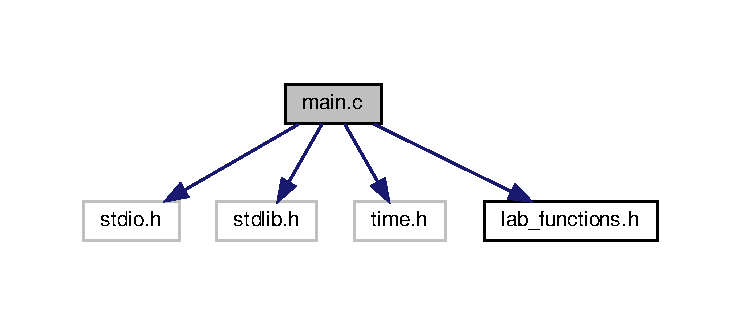
\includegraphics[width=350pt]{main_8c__incl}
\end{center}
\end{figure}
\subsection*{Макровизначення}
\begin{DoxyCompactItemize}
\item 
\#define \hyperlink{main_8c_aff606fb64ff89d5982673319bab86b19}{clear}()~printf(\char`\"{}\textbackslash{}033\mbox{[}H\textbackslash{}033\mbox{[}J\char`\"{})
\end{DoxyCompactItemize}
\subsection*{Функції}
\begin{DoxyCompactItemize}
\item 
char $\ast$ \hyperlink{main_8c_a638293d509eded9d6ef7552ae1b17f2b}{message\+\_\+input} (char message\mbox{[}$\,$\mbox{]})
\begin{DoxyCompactList}\small\item\em Отримує від користувача ввід, перед яким виводить повідомлення \end{DoxyCompactList}\item 
int \hyperlink{main_8c_a9594b83ee908d195f5ff508da5c23c58}{is\+\_\+every\+\_\+digit} (char $\ast$str)
\begin{DoxyCompactList}\small\item\em Перевірка чи кожне введене число є десятковим (від\textquotesingle{}ємним також) \end{DoxyCompactList}\item 
int \hyperlink{main_8c_a5d7849c249859dd438a37f1e6e5adf70}{is\+\_\+every\+\_\+digit\+\_\+double} (char $\ast$str)
\begin{DoxyCompactList}\small\item\em Перевірка чи кожне введене число є дробовим (від\textquotesingle{}ємним також) \end{DoxyCompactList}\item 
void \hyperlink{main_8c_a770281b98587f9f65ca4cc75b1d061db}{to\+\_\+repeat} (void($\ast$func)(void), char message\mbox{[}$\,$\mbox{]})
\begin{DoxyCompactList}\small\item\em Функція, що повторює задану їй функцію за бажанням користувача. \end{DoxyCompactList}\item 
long \hyperlink{main_8c_a50be0d9d5898cd1c9b3a07abb78faf4e}{pow\+\_\+10\+\_\+to} (int $\ast$power)
\begin{DoxyCompactList}\small\item\em Повертає 10 в заданому степені \end{DoxyCompactList}\item 
void \hyperlink{main_8c_a6f453bc035d85e967bd5032eca31a155}{input\+\_\+int} (char message\mbox{[}$\,$\mbox{]}, int $\ast$number, int lwr\+\_\+border, int hir\+\_\+border)
\begin{DoxyCompactList}\small\item\em Реалізація корректного введення цілих десяткових чисел користувачем \end{DoxyCompactList}\item 
void \hyperlink{main_8c_ac835db5eadbfefce4a51eae30806a486}{input\+\_\+long\+\_\+double} (char message\mbox{[}$\,$\mbox{]}, long double $\ast$number, long double lwr\+\_\+border, long double hir\+\_\+border)
\begin{DoxyCompactList}\small\item\em Реалізація корректного введення десяткових дійсних чисел користувачем \end{DoxyCompactList}\item 
long double \hyperlink{main_8c_a41a04980c21ff33f1bfb435f275011db}{round\+\_\+number} (long double $\ast$num, int $\ast$precision)
\begin{DoxyCompactList}\small\item\em Заокруглює число за математичними правилами з заданою точністю \end{DoxyCompactList}\item 
void \hyperlink{main_8c_a2f5dd4f3afe9bea7f6dd19ed24cd9d16}{print\+\_\+dividers} (int $\ast$entered\+\_\+number)
\begin{DoxyCompactList}\small\item\em Виводить усі множники числа \end{DoxyCompactList}\item 
int \hyperlink{main_8c_a39c41664490ca73a6f8b8224e1191711}{count\+\_\+length} (char phrase\mbox{[}$\,$\mbox{]}, int i)
\begin{DoxyCompactList}\small\item\em Рекурсивно рахує довжину рядка \end{DoxyCompactList}\item 
int \hyperlink{main_8c_a48523aba9a802fbdca6e9670a036253c}{get\+\_\+length} (char phrase\mbox{[}$\,$\mbox{]})
\item 
void \hyperlink{main_8c_a2e10594dc040249a898e2880b4c64322}{task\+\_\+1} ()
\begin{DoxyCompactList}\small\item\em Вибір підзавдання №1. \end{DoxyCompactList}\item 
void \hyperlink{main_8c_a40968dfe24ede22947096429f30444a4}{task\+\_\+1\+\_\+1} ()
\begin{DoxyCompactList}\small\item\em Виконання завдання №1 підзавдання №1. \end{DoxyCompactList}\item 
void \hyperlink{main_8c_a97a9145d16ec992fa06404b068bd4e18}{task\+\_\+1\+\_\+2} ()
\begin{DoxyCompactList}\small\item\em Виконання завдання №1 підзавдання №2. \end{DoxyCompactList}\item 
void \hyperlink{main_8c_a08570886a32f0508e2a3f23c4ea06339}{task\+\_\+2} ()
\begin{DoxyCompactList}\small\item\em Виконання завдання №2. \end{DoxyCompactList}\item 
\mbox{\Hypertarget{main_8c_ae66f6b31b5ad750f1fe042a706a4e3d4}\label{main_8c_ae66f6b31b5ad750f1fe042a706a4e3d4}} 
int {\bfseries main} ()
\end{DoxyCompactItemize}


\subsection{Опис макровизначень}
\mbox{\Hypertarget{main_8c_aff606fb64ff89d5982673319bab86b19}\label{main_8c_aff606fb64ff89d5982673319bab86b19}} 
\index{main.\+c@{main.\+c}!clear@{clear}}
\index{clear@{clear}!main.\+c@{main.\+c}}
\subsubsection{\texorpdfstring{clear}{clear}}
{\footnotesize\ttfamily \#define clear(\begin{DoxyParamCaption}{ }\end{DoxyParamCaption})~printf(\char`\"{}\textbackslash{}033\mbox{[}H\textbackslash{}033\mbox{[}J\char`\"{})}

Очищення екрану на U\+N\+IX системах 

\subsection{Опис функцій}
\mbox{\Hypertarget{main_8c_a39c41664490ca73a6f8b8224e1191711}\label{main_8c_a39c41664490ca73a6f8b8224e1191711}} 
\index{main.\+c@{main.\+c}!count\+\_\+length@{count\+\_\+length}}
\index{count\+\_\+length@{count\+\_\+length}!main.\+c@{main.\+c}}
\subsubsection{\texorpdfstring{count\+\_\+length()}{count\_length()}}
{\footnotesize\ttfamily int count\+\_\+length (\begin{DoxyParamCaption}\item[{char}]{phrase\mbox{[}$\,$\mbox{]},  }\item[{int}]{i }\end{DoxyParamCaption})}



Рекурсивно рахує довжину рядка 


\begin{DoxyParams}{Аргументи}
{\em phrase} & Власне рядок \\
\hline
{\em i} & Лічильник \\
\hline
\end{DoxyParams}
\begin{DoxyReturn}{Повертає}
Довжину рядка 
\end{DoxyReturn}
Сумуєм цей символ з символами решти рядка до кінця.
\begin{DoxyCode}
285                                      \{
289     \textcolor{keywordflow}{if} (!phrase[i])\{
290         \textcolor{keywordflow}{return} 0;
291     \}
292     \textcolor{keywordtype}{int} sum = 1 + \hyperlink{main_8c_a39c41664490ca73a6f8b8224e1191711}{count\_length}(phrase,i+1);
293     \textcolor{keywordflow}{return} sum;
294 \}
\end{DoxyCode}
\mbox{\Hypertarget{main_8c_a48523aba9a802fbdca6e9670a036253c}\label{main_8c_a48523aba9a802fbdca6e9670a036253c}} 
\index{main.\+c@{main.\+c}!get\+\_\+length@{get\+\_\+length}}
\index{get\+\_\+length@{get\+\_\+length}!main.\+c@{main.\+c}}
\subsubsection{\texorpdfstring{get\+\_\+length()}{get\_length()}}
{\footnotesize\ttfamily int get\+\_\+length (\begin{DoxyParamCaption}\item[{char}]{phrase\mbox{[}$\,$\mbox{]} }\end{DoxyParamCaption})}

Обгортка для \hyperlink{main_8c_a39c41664490ca73a6f8b8224e1191711}{count\+\_\+length()} \hyperlink{main_8c_a48523aba9a802fbdca6e9670a036253c}{get\+\_\+length()} -\/ обгортка для \hyperlink{main_8c_a39c41664490ca73a6f8b8224e1191711}{count\+\_\+length()} без задання лишньої константи. Виконуєм рекурсивну функцію підрахунку дожвжини рядка \hyperlink{main_8c_a39c41664490ca73a6f8b8224e1191711}{count\+\_\+length()} починаючи з 0.
\begin{DoxyCode}
268                              \{
274     \textcolor{keywordflow}{return} \hyperlink{main_8c_a39c41664490ca73a6f8b8224e1191711}{count\_length}(phrase,0);
275 \}
\end{DoxyCode}
\mbox{\Hypertarget{main_8c_a6f453bc035d85e967bd5032eca31a155}\label{main_8c_a6f453bc035d85e967bd5032eca31a155}} 
\index{main.\+c@{main.\+c}!input\+\_\+int@{input\+\_\+int}}
\index{input\+\_\+int@{input\+\_\+int}!main.\+c@{main.\+c}}
\subsubsection{\texorpdfstring{input\+\_\+int()}{input\_int()}}
{\footnotesize\ttfamily void input\+\_\+int (\begin{DoxyParamCaption}\item[{char}]{message\mbox{[}$\,$\mbox{]},  }\item[{int $\ast$}]{number,  }\item[{int}]{lwr\+\_\+border,  }\item[{int}]{hir\+\_\+border }\end{DoxyParamCaption})}



Реалізація корректного введення цілих десяткових чисел користувачем 


\begin{DoxyParams}{Аргументи}
{\em message} & Повідомлення до користувача \\
\hline
{\em number} & Змінна в яку буде записуватися правильний ввід \\
\hline
{\em lwr\+\_\+border} & Нижня межа \\
\hline
{\em hir\+\_\+border} & Верхня межа \\
\hline
\end{DoxyParams}
Перевіряєм на належність типу та межам
\begin{DoxyCode}
241                                                                           \{
245     \textcolor{keywordflow}{if} (lwr\_border == hir\_border)\{
246         lwr\_border = INT\_MIN;
247         hir\_border = INT\_MAX;
248     \}
249     \textcolor{keywordtype}{char} *usr\_input = \hyperlink{main_8c_a638293d509eded9d6ef7552ae1b17f2b}{message\_input}(message);
250     \textcolor{keywordtype}{int} is\_suits = sscanf(usr\_input,\textcolor{stringliteral}{"%d"},number);
251     \textcolor{keywordflow}{while} (!is\_suits || !\hyperlink{main_8c_a9594b83ee908d195f5ff508da5c23c58}{is\_every\_digit}(usr\_input) || *number < lwr\_border || *number > 
      hir\_border)\{
252         printf(\textcolor{stringliteral}{"ERROR INPUT\(\backslash\)n"});
253         usr\_input = \hyperlink{main_8c_a638293d509eded9d6ef7552ae1b17f2b}{message\_input}(message);
254         is\_suits = sscanf(usr\_input,\textcolor{stringliteral}{"%d"},number);
255     \}
256 \}
\end{DoxyCode}
\mbox{\Hypertarget{main_8c_ac835db5eadbfefce4a51eae30806a486}\label{main_8c_ac835db5eadbfefce4a51eae30806a486}} 
\index{main.\+c@{main.\+c}!input\+\_\+long\+\_\+double@{input\+\_\+long\+\_\+double}}
\index{input\+\_\+long\+\_\+double@{input\+\_\+long\+\_\+double}!main.\+c@{main.\+c}}
\subsubsection{\texorpdfstring{input\+\_\+long\+\_\+double()}{input\_long\_double()}}
{\footnotesize\ttfamily void input\+\_\+long\+\_\+double (\begin{DoxyParamCaption}\item[{char}]{message\mbox{[}$\,$\mbox{]},  }\item[{long double $\ast$}]{number,  }\item[{long double}]{lwr\+\_\+border,  }\item[{long double}]{hir\+\_\+border }\end{DoxyParamCaption})}



Реалізація корректного введення десяткових дійсних чисел користувачем 


\begin{DoxyParams}{Аргументи}
{\em message} & Повідомлення до користувача \\
\hline
{\em number} & Змінна в яку буде записуватися правильний ввід \\
\hline
{\em lwr\+\_\+border} & Нижня межа \\
\hline
{\em hir\+\_\+border} & Верхня межа \\
\hline
\end{DoxyParams}
Перевіряєм на належність типу та межам
\begin{DoxyCode}
121                                                                                                           \{
125     \textcolor{keywordflow}{if} (lwr\_border == hir\_border)\{
126         lwr\_border = LDBL\_MIN;
127         hir\_border = LDBL\_MAX;
128     \}
129     \textcolor{keywordtype}{char} *usr\_input = \hyperlink{main_8c_a638293d509eded9d6ef7552ae1b17f2b}{message\_input}(message);
130     \textcolor{keywordtype}{int} is\_suits = sscanf(usr\_input,\textcolor{stringliteral}{"%Lf"},number);
131     \textcolor{keywordflow}{while} (!is\_suits || (!\hyperlink{main_8c_a5d7849c249859dd438a37f1e6e5adf70}{is\_every\_digit\_double}(usr\_input) && !
      \hyperlink{main_8c_a9594b83ee908d195f5ff508da5c23c58}{is\_every\_digit}(usr\_input)) || *number < lwr\_border || *number > hir\_border)\{
132         printf(\textcolor{stringliteral}{"ERROR INPUT\(\backslash\)n"});
133         usr\_input = \hyperlink{main_8c_a638293d509eded9d6ef7552ae1b17f2b}{message\_input}(message);
134         is\_suits = sscanf(usr\_input,\textcolor{stringliteral}{"%Lf"},number);
135     \}
136 \}
\end{DoxyCode}
\mbox{\Hypertarget{main_8c_a9594b83ee908d195f5ff508da5c23c58}\label{main_8c_a9594b83ee908d195f5ff508da5c23c58}} 
\index{main.\+c@{main.\+c}!is\+\_\+every\+\_\+digit@{is\+\_\+every\+\_\+digit}}
\index{is\+\_\+every\+\_\+digit@{is\+\_\+every\+\_\+digit}!main.\+c@{main.\+c}}
\subsubsection{\texorpdfstring{is\+\_\+every\+\_\+digit()}{is\_every\_digit()}}
{\footnotesize\ttfamily int is\+\_\+every\+\_\+digit (\begin{DoxyParamCaption}\item[{char $\ast$}]{str }\end{DoxyParamCaption})}



Перевірка чи кожне введене число є десятковим (від\textquotesingle{}ємним також) 


\begin{DoxyParams}{Аргументи}
{\em str} & число у вигляді увеного масиву char \\
\hline
\end{DoxyParams}
\begin{DoxyReturn}{Повертає}
1, якщо число десяткове, 0 якщо ні 
\end{DoxyReturn}
Преревіряєм кожен символ на те, чи є він числом. Дозволяються від\textquotesingle{}ємні числа.
\begin{DoxyCode}
202                              \{
207     \textcolor{keywordtype}{int} len = strlen(str);
208     \textcolor{keywordtype}{int} i = 0;
209     \textcolor{keywordflow}{if} (atoi(str)<0) i++;\textcolor{comment}{// якщо менше нуля - мінус пропускаєм}
210     \textcolor{keywordflow}{for} (i; i < len-1; ++i) \{
211         \textcolor{keywordflow}{if} (!isdigit(str[i]))\{
212             \textcolor{keywordflow}{return} 0;\textcolor{comment}{//будь-який знак - не цифра}
213         \}
214     \}
215     \textcolor{keywordflow}{return} 1;
216 \}
\end{DoxyCode}
\mbox{\Hypertarget{main_8c_a5d7849c249859dd438a37f1e6e5adf70}\label{main_8c_a5d7849c249859dd438a37f1e6e5adf70}} 
\index{main.\+c@{main.\+c}!is\+\_\+every\+\_\+digit\+\_\+double@{is\+\_\+every\+\_\+digit\+\_\+double}}
\index{is\+\_\+every\+\_\+digit\+\_\+double@{is\+\_\+every\+\_\+digit\+\_\+double}!main.\+c@{main.\+c}}
\subsubsection{\texorpdfstring{is\+\_\+every\+\_\+digit\+\_\+double()}{is\_every\_digit\_double()}}
{\footnotesize\ttfamily int is\+\_\+every\+\_\+digit\+\_\+double (\begin{DoxyParamCaption}\item[{char $\ast$}]{str }\end{DoxyParamCaption})}



Перевірка чи кожне введене число є дробовим (від\textquotesingle{}ємним також) 


\begin{DoxyParams}{Аргументи}
{\em str} & число у вигляді увеного масиву char \\
\hline
\end{DoxyParams}
\begin{DoxyReturn}{Повертає}
1, якщо число дробове, 0 якщо ні 
\end{DoxyReturn}
Зчитуєм число та перевіряєм чи є воно дійсним та чи не є у нього нічого окрім цифр, знака мінус, однієї крапки
\begin{DoxyCode}
218                                     \{
223     \textcolor{keywordtype}{int} len = strlen(str);
224     \textcolor{keywordtype}{long} \textcolor{keywordtype}{double} number;
225     sscanf(str,\textcolor{stringliteral}{"%Lf"},&number);
226     \textcolor{keywordtype}{int} i = 0, dot\_counter = 0;
227     \textcolor{keywordflow}{if} (number<0.0) i++;\textcolor{comment}{// якщо менше нуля - мінус пропускаєм}
228     \textcolor{keywordflow}{for} (i; i < len-1; ++i) \{
229         \textcolor{keywordflow}{if} (!isdigit(str[i]))\{
230             \textcolor{keywordflow}{if} (str[i]==\textcolor{charliteral}{'.'}) \{
231                 dot\_counter++;
232             \}\textcolor{keywordflow}{else}\{
233                 \textcolor{keywordflow}{return} 0;\textcolor{comment}{//будь-який знак - не цифра або крапка (максимум 1)}
234             \}
235         \}
236     \}
237     \textcolor{keywordflow}{if} (dot\_counter-1) \textcolor{keywordflow}{return} 0;
238     \textcolor{keywordflow}{return} 1;
239 \}
\end{DoxyCode}
\mbox{\Hypertarget{main_8c_a638293d509eded9d6ef7552ae1b17f2b}\label{main_8c_a638293d509eded9d6ef7552ae1b17f2b}} 
\index{main.\+c@{main.\+c}!message\+\_\+input@{message\+\_\+input}}
\index{message\+\_\+input@{message\+\_\+input}!main.\+c@{main.\+c}}
\subsubsection{\texorpdfstring{message\+\_\+input()}{message\_input()}}
{\footnotesize\ttfamily char $\ast$ message\+\_\+input (\begin{DoxyParamCaption}\item[{char}]{message\mbox{[}$\,$\mbox{]} }\end{DoxyParamCaption})}



Отримує від користувача ввід, перед яким виводить повідомлення 


\begin{DoxyParams}{Аргументи}
{\em message} & Повідомлення, яке буде показане користувачу \\
\hline
\end{DoxyParams}
\begin{DoxyReturn}{Повертає}
Ввід користувача в форматі {\ttfamily char}\mbox{[}\mbox{]} 
\end{DoxyReturn}

\begin{DoxyCode}
195                                    \{
196     \textcolor{keywordtype}{char} *usr\_input = (\textcolor{keywordtype}{char}*) malloc(\textcolor{keyword}{sizeof}(\textcolor{keywordtype}{char})*254);
197     printf(\textcolor{stringliteral}{"%s"}, message); \textcolor{comment}{// Виводимо повідомлення користувачу}
198     fgets(usr\_input, 254, stdin);
199     \textcolor{keywordflow}{return} usr\_input;
200 \}
\end{DoxyCode}
\mbox{\Hypertarget{main_8c_a50be0d9d5898cd1c9b3a07abb78faf4e}\label{main_8c_a50be0d9d5898cd1c9b3a07abb78faf4e}} 
\index{main.\+c@{main.\+c}!pow\+\_\+10\+\_\+to@{pow\+\_\+10\+\_\+to}}
\index{pow\+\_\+10\+\_\+to@{pow\+\_\+10\+\_\+to}!main.\+c@{main.\+c}}
\subsubsection{\texorpdfstring{pow\+\_\+10\+\_\+to()}{pow\_10\_to()}}
{\footnotesize\ttfamily long pow\+\_\+10\+\_\+to (\begin{DoxyParamCaption}\item[{int $\ast$}]{power }\end{DoxyParamCaption})}



Повертає 10 в заданому степені 

Код наведений нижче 
\begin{DoxyParams}{Аргументи}
{\em power} & Степінь десятки \\
\hline
\end{DoxyParams}
\begin{DoxyReturn}{Повертає}
10$^\wedge$power 
\end{DoxyReturn}

\begin{DoxyCode}
277                           \{
278 
279     \textcolor{keywordtype}{long} ten = 1;
280     \textcolor{keywordflow}{for} (\textcolor{keywordtype}{int} i = 0; i < *power; ++i) \{
281         ten *= 10;
282     \}
283     \textcolor{keywordflow}{return} ten;
284 \}
\end{DoxyCode}
\mbox{\Hypertarget{main_8c_a2f5dd4f3afe9bea7f6dd19ed24cd9d16}\label{main_8c_a2f5dd4f3afe9bea7f6dd19ed24cd9d16}} 
\index{main.\+c@{main.\+c}!print\+\_\+dividers@{print\+\_\+dividers}}
\index{print\+\_\+dividers@{print\+\_\+dividers}!main.\+c@{main.\+c}}
\subsubsection{\texorpdfstring{print\+\_\+dividers()}{print\_dividers()}}
{\footnotesize\ttfamily void print\+\_\+dividers (\begin{DoxyParamCaption}\item[{int $\ast$}]{entered\+\_\+number }\end{DoxyParamCaption})}



Виводить усі множники числа 


\begin{DoxyParams}{Аргументи}
{\em entered\+\_\+number} & Число, з якого берем множники \\
\hline
\end{DoxyParams}
Просто ідемо від одиниці до заданого числа і якщо це дільник -\/ виводим. Також виводим тривіальні дільники.
\begin{DoxyCode}
296                                         \{
301     printf(\textcolor{stringliteral}{"Дільники числа:\(\backslash\)n1\(\backslash\)n"});
302     \textcolor{keywordflow}{for} (\textcolor{keywordtype}{int} i = 2; i < *entered\_number/2; ++i) \{
303         \textcolor{keywordflow}{if} (!(*entered\_number%i))\{
304             printf(\textcolor{stringliteral}{"%d\(\backslash\)n"}, i);
305         \}
306     \}
307     \textcolor{keywordflow}{if} (*entered\_number>1) printf(\textcolor{stringliteral}{"%d\(\backslash\)n"},*entered\_number);
308 \}
\end{DoxyCode}
\mbox{\Hypertarget{main_8c_a41a04980c21ff33f1bfb435f275011db}\label{main_8c_a41a04980c21ff33f1bfb435f275011db}} 
\index{main.\+c@{main.\+c}!round\+\_\+number@{round\+\_\+number}}
\index{round\+\_\+number@{round\+\_\+number}!main.\+c@{main.\+c}}
\subsubsection{\texorpdfstring{round\+\_\+number()}{round\_number()}}
{\footnotesize\ttfamily long double round\+\_\+number (\begin{DoxyParamCaption}\item[{long double $\ast$}]{num,  }\item[{int $\ast$}]{precision }\end{DoxyParamCaption})}



Заокруглює число за математичними правилами з заданою точністю 


\begin{DoxyParams}{Аргументи}
{\em num} & Число, яке необхідно заокруглити \\
\hline
{\em precision} & Точність \\
\hline
\end{DoxyParams}
\begin{DoxyReturn}{Повертає}
Заокруглене число 
\end{DoxyReturn}
Створюєм значення точності перетворене в десятки {\ttfamily accuracy}. {\ttfamily math\+\_\+round\+\_\+addition} використовуєтся заокруглення за математичними правилами (= \mbox{[}x+0.5\mbox{]}). Відкидається решта знаків після заданої точності. {\ttfamily answer} перетворюється за заданою точністю в long double
\begin{DoxyCode}
310                                                            \{
317     \textcolor{comment}{// створено додаткові змінні для пояснення суті та полегшення відладки}
318     \textcolor{keywordtype}{long} accuracy = \hyperlink{main_8c_a50be0d9d5898cd1c9b3a07abb78faf4e}{pow\_10\_to}(precision); \textcolor{comment}{// значення точності перетворене в десятки}
319     \textcolor{keywordtype}{long} \textcolor{keywordtype}{double} math\_round\_addition = 0.5*(1/(\textcolor{keywordtype}{long} double)accuracy);\textcolor{comment}{// використовуєтся заокруглення за
       математичними правилами (= [x+0.5])}
320     \textcolor{keywordtype}{long} \textcolor{keywordtype}{double} answer = (long)(((*num)+math\_round\_addition)*accuracy);\textcolor{comment}{// відкидаються решта "нулів"}
321     answer /= (\textcolor{keywordtype}{long} double)accuracy ;\textcolor{comment}{// власне поділ на цілу і дробову частини}
322     \textcolor{keywordflow}{return} answer;
323 \}
\end{DoxyCode}
\mbox{\Hypertarget{main_8c_a2e10594dc040249a898e2880b4c64322}\label{main_8c_a2e10594dc040249a898e2880b4c64322}} 
\index{main.\+c@{main.\+c}!task\+\_\+1@{task\+\_\+1}}
\index{task\+\_\+1@{task\+\_\+1}!main.\+c@{main.\+c}}
\subsubsection{\texorpdfstring{task\+\_\+1()}{task\_1()}}
{\footnotesize\ttfamily void task\+\_\+1 (\begin{DoxyParamCaption}{ }\end{DoxyParamCaption})}



Вибір підзавдання №1. 

Код функції нижче 
\begin{DoxyCode}
137              \{
138     \textcolor{keywordtype}{int} choice;
139     \textcolor{keywordflow}{do} \{
140         \hyperlink{main_8c_aff606fb64ff89d5982673319bab86b19}{clear}();
141         \hyperlink{main_8c_a6f453bc035d85e967bd5032eca31a155}{input\_int}(\textcolor{stringliteral}{"Виберіть номер підзавдання (1, 2):\(\backslash\)n"},
142                   &choice,
143                   1,
144                   2);
145         \textcolor{keywordflow}{switch} (choice) \{
146             \textcolor{keywordflow}{case} 1:
147                 \hyperlink{main_8c_a770281b98587f9f65ca4cc75b1d061db}{to\_repeat}(\hyperlink{main_8c_a40968dfe24ede22947096429f30444a4}{task\_1\_1},\textcolor{stringliteral}{"Бажаєте продовжити виконання підзавдання 1?"});
148                 \textcolor{keywordflow}{break};
149             \textcolor{keywordflow}{case} 2:
150                 \hyperlink{main_8c_a770281b98587f9f65ca4cc75b1d061db}{to\_repeat}(\hyperlink{main_8c_a97a9145d16ec992fa06404b068bd4e18}{task\_1\_2}, \textcolor{stringliteral}{"Бажаєте продовжити виконання підзавдання 2?"});
151                 \textcolor{keywordflow}{break};
152         \}
153         \hyperlink{main_8c_a6f453bc035d85e967bd5032eca31a155}{input\_int}(\textcolor{stringliteral}{"Бажаєте повторно виконати вибір підзавдання завдання 1?:\(\backslash\)n"}, &choice, 0, 1);
154     \}\textcolor{keywordflow}{while} (choice);
155 \}
\end{DoxyCode}
\mbox{\Hypertarget{main_8c_a40968dfe24ede22947096429f30444a4}\label{main_8c_a40968dfe24ede22947096429f30444a4}} 
\index{main.\+c@{main.\+c}!task\+\_\+1\+\_\+1@{task\+\_\+1\+\_\+1}}
\index{task\+\_\+1\+\_\+1@{task\+\_\+1\+\_\+1}!main.\+c@{main.\+c}}
\subsubsection{\texorpdfstring{task\+\_\+1\+\_\+1()}{task\_1\_1()}}
{\footnotesize\ttfamily void task\+\_\+1\+\_\+1 (\begin{DoxyParamCaption}{ }\end{DoxyParamCaption})}



Виконання завдання №1 підзавдання №1. 

Уводим вхідні дані за допомогою функцій, що підтримують валідацію \hyperlink{main_8c_ac835db5eadbfefce4a51eae30806a486}{input\+\_\+long\+\_\+double()} \hyperlink{main_8c_a6f453bc035d85e967bd5032eca31a155}{input\+\_\+int()} .~\newline
Викликаєм власну функцію заокруглення \hyperlink{main_8c_a41a04980c21ff33f1bfb435f275011db}{round\+\_\+number()} . Виводим число з заданою точністю
\begin{DoxyCode}
156                \{
163     printf(\textcolor{stringliteral}{"Завдання 1.1\(\backslash\)n"});
164     \textcolor{keywordtype}{long} \textcolor{keywordtype}{double} entered\_number;
165     \textcolor{keywordtype}{int} precision;
166     \hyperlink{main_8c_ac835db5eadbfefce4a51eae30806a486}{input\_long\_double}(\textcolor{stringliteral}{"Введіть дійсне число\(\backslash\)n"}, &entered\_number, 0.0, 0.0);
167     \hyperlink{main_8c_a6f453bc035d85e967bd5032eca31a155}{input\_int}(\textcolor{stringliteral}{"Введіть бажану точність\(\backslash\)n"}, &precision, 0, INT\_MAX);
168     \textcolor{keywordtype}{long} \textcolor{keywordtype}{double} num = \hyperlink{main_8c_a41a04980c21ff33f1bfb435f275011db}{round\_number}(&entered\_number, &precision);
169     printf(\textcolor{stringliteral}{"%.*Lf\(\backslash\)n"}, precision, num);
170 \}
\end{DoxyCode}
\mbox{\Hypertarget{main_8c_a97a9145d16ec992fa06404b068bd4e18}\label{main_8c_a97a9145d16ec992fa06404b068bd4e18}} 
\index{main.\+c@{main.\+c}!task\+\_\+1\+\_\+2@{task\+\_\+1\+\_\+2}}
\index{task\+\_\+1\+\_\+2@{task\+\_\+1\+\_\+2}!main.\+c@{main.\+c}}
\subsubsection{\texorpdfstring{task\+\_\+1\+\_\+2()}{task\_1\_2()}}
{\footnotesize\ttfamily void task\+\_\+1\+\_\+2 (\begin{DoxyParamCaption}{ }\end{DoxyParamCaption})}



Виконання завдання №1 підзавдання №2. 

Уводим вхідні дані за допомогою функцій, що підтримують валідацію \hyperlink{main_8c_a6f453bc035d85e967bd5032eca31a155}{input\+\_\+int()} .~\newline
Виводимо дільники за допомогою \hyperlink{main_8c_a2f5dd4f3afe9bea7f6dd19ed24cd9d16}{print\+\_\+dividers()} .
\begin{DoxyCode}
171                \{
177     printf(\textcolor{stringliteral}{"Завдання 1.2\(\backslash\)n"});
178     \textcolor{keywordtype}{int} entered\_number;
179     \hyperlink{main_8c_a6f453bc035d85e967bd5032eca31a155}{input\_int}(\textcolor{stringliteral}{"Уведіть ціле додатнє число\(\backslash\)n"},&entered\_number,1,INT\_MAX);
180     \hyperlink{main_8c_a2f5dd4f3afe9bea7f6dd19ed24cd9d16}{print\_dividers}(&entered\_number);
181 \}
\end{DoxyCode}
\mbox{\Hypertarget{main_8c_a08570886a32f0508e2a3f23c4ea06339}\label{main_8c_a08570886a32f0508e2a3f23c4ea06339}} 
\index{main.\+c@{main.\+c}!task\+\_\+2@{task\+\_\+2}}
\index{task\+\_\+2@{task\+\_\+2}!main.\+c@{main.\+c}}
\subsubsection{\texorpdfstring{task\+\_\+2()}{task\_2()}}
{\footnotesize\ttfamily void task\+\_\+2 (\begin{DoxyParamCaption}{ }\end{DoxyParamCaption})}



Виконання завдання №2. 

Вводимо фразу латиницею. Обчислюємо довжину рядка за допомогою \hyperlink{main_8c_a48523aba9a802fbdca6e9670a036253c}{get\+\_\+length()} та віднімаєм символ переходу на новий рядок. Виводим довжину.
\begin{DoxyCode}
183              \{
188     printf(\textcolor{stringliteral}{"Завдання 2\(\backslash\)n"});
189     \textcolor{keywordtype}{char} phrase[254];
190     printf(\textcolor{stringliteral}{"Введіть фразу (тільки латиниця (ASCII), інакше - невірний результат)\(\backslash\)n"});
191     fgets(phrase, 253, stdin);
192     printf(\textcolor{stringliteral}{"Її довжина = %d\(\backslash\)n"}, \hyperlink{main_8c_a48523aba9a802fbdca6e9670a036253c}{get\_length}(phrase)-1);
193 \}
\end{DoxyCode}
\mbox{\Hypertarget{main_8c_a770281b98587f9f65ca4cc75b1d061db}\label{main_8c_a770281b98587f9f65ca4cc75b1d061db}} 
\index{main.\+c@{main.\+c}!to\+\_\+repeat@{to\+\_\+repeat}}
\index{to\+\_\+repeat@{to\+\_\+repeat}!main.\+c@{main.\+c}}
\subsubsection{\texorpdfstring{to\+\_\+repeat()}{to\_repeat()}}
{\footnotesize\ttfamily void to\+\_\+repeat (\begin{DoxyParamCaption}\item[{void($\ast$)(void)}]{func,  }\item[{char}]{message\mbox{[}$\,$\mbox{]} }\end{DoxyParamCaption})}



Функція, що повторює задану їй функцію за бажанням користувача. 


\begin{DoxyParams}{Аргументи}
{\em func} & Функція, яка буде повторюватись \\
\hline
{\em message} & Повідомлення до користувача \\
\hline
{\em pow\+\_\+10\+\_\+to} & \\
\hline
\end{DoxyParams}
Викорисковуються вказівники на функцію, щоб забезпечити її повторне виконання.
\begin{DoxyCode}
257                                                   \{
262     \textcolor{keywordtype}{int} choice;
263     \textcolor{keywordflow}{do}\{
264         (*func)();
265         \hyperlink{main_8c_a6f453bc035d85e967bd5032eca31a155}{input\_int}(message,&choice,0,1);
266     \}\textcolor{keywordflow}{while} (choice);
267 \}
\end{DoxyCode}

%--- End generated contents ---

% Index
\backmatter
\newpage
\phantomsection
\clearemptydoublepage
\addcontentsline{toc}{chapter}{Предметний покажчик}
\printindex

\end{document}
